

\documentclass{svproc}
\usepackage[english]{babel} % English language/hyphenation
%\usepackage{amsmath,amsfonts,amsthm} % Math packages
\usepackage{url}
\usepackage{sectsty} % Allows customizing section commands
\usepackage{graphicx}
\usepackage{multicol}
\usepackage{footmisc}
%\usepackage{cite}
\bibliographystyle{unsrt}

%----------------------------------------------------------------------------------------
%	TITLE SECTION
%----------------------------------------------------------------------------------------

\newcommand{\horrule}[1]{\rule{\linewidth}{#1}} % Create horizontal rule command with 1 argument of height

\title{An Introduction of Time Domain Numerical Methods for Faster Acoustic Modelling} % The assignment title
\titlerunning{Time Domain Methods for Faster Acoustic Modelling}
\author{Simon Durbridge} % Your name
\authorrunning{S.Durbridge}
%\date{\normalsize\today} % Today's date or a custom date
\institute{Dept. Engineering, Mathematics \&\ Computing\\ University of Derby\\
\email{s.durbridge1@unimail.derby.ac.uk} % optional, same for URL of homepage
} % end of address field

\begin{document}

\maketitle % Print the title

%----------------------------------------------------------------------------------------
%	Abstract
%----------------------------------------------------------------------------------------

\begin{abstract}
Wave based acoustic modelling methods promise many benefits over ray based methods, though have considerable computational cost. For real-time applications time domain wave solving may be of particular use, due to scalability and handling of sources and receivers in the problem. Two potential methods of reducing computation time of the finite difference time domain method may be developed for applications that require real time solutions. The pseudospectral time domain and sparse finite difference methods for acoustics are introduced within the report, along with a background to acoustic modelling, ray based and wave based modelling methods. 


\keywords{Acoustic Modelling, Numerical Methods, Time Domain, Fast}
\end{abstract}

%----------------------------------------------------------------------------------------
%	Contents
%----------------------------------------------------------------------------------------

%\tableofcontents

%\newpage

%----------------------------------------------------------------------------------------
%	Figures
%----------------------------------------------------------------------------------------

%\listoffigures

%\newpage



%----------------------------------------------------------------------------------------
%	Introduction
%----------------------------------------------------------------------------------------

\section{Introduction}
Interest in acoustic modelling continues to increase due to external factors such as a renewed focus in global standards of distributed loudspeaker system design~\cite{BritishStandardsInst2013}, as well as trends in consumer technology such as the video games and entertainment applications~\cite{Google2016}. This brings acoustic simulation to the forefront for areas such as public address and safety(Public Address Voice Alarm(PAVA))system design, as well as less safety driven interests such as immersive virtual reality experiences of synthesized spaces for entertainment. The benefits of improved acoustic modelling methods allow key stakeholders to leverage high quality results and create better quality products~\cite{Dod2016}. Time is an ever more strict constraint in many commercial development applications, and an inherent issue with high accuracy modelling is a significant increase in time spent simulating, as well as computational resources and a requirement for specialist knowledge.\\

\subsection{Problem Definition}
Real time acoustic modelling could be of significant benefit to many applications; Engineers could make design changes and see results 'on the fly', and entertainment users could have more realistic experiences. These benefits should be possible for an arbitrary number of sources and receivers, in proportionally large environments with high quality results. Is it possible to further reduce computation time for simulations of large acoustic problems, to provide results in real time for the full human audio frequency range? There are two 'branches' of computation solution that should be considered: the direct solution i.e. direct outputs or audio samples from the simulation, and indirect solutions i.e. a system impulse response that may be convolved with mixed source signals in order to create an auralization of the system.//


\begin{figure}
\centering
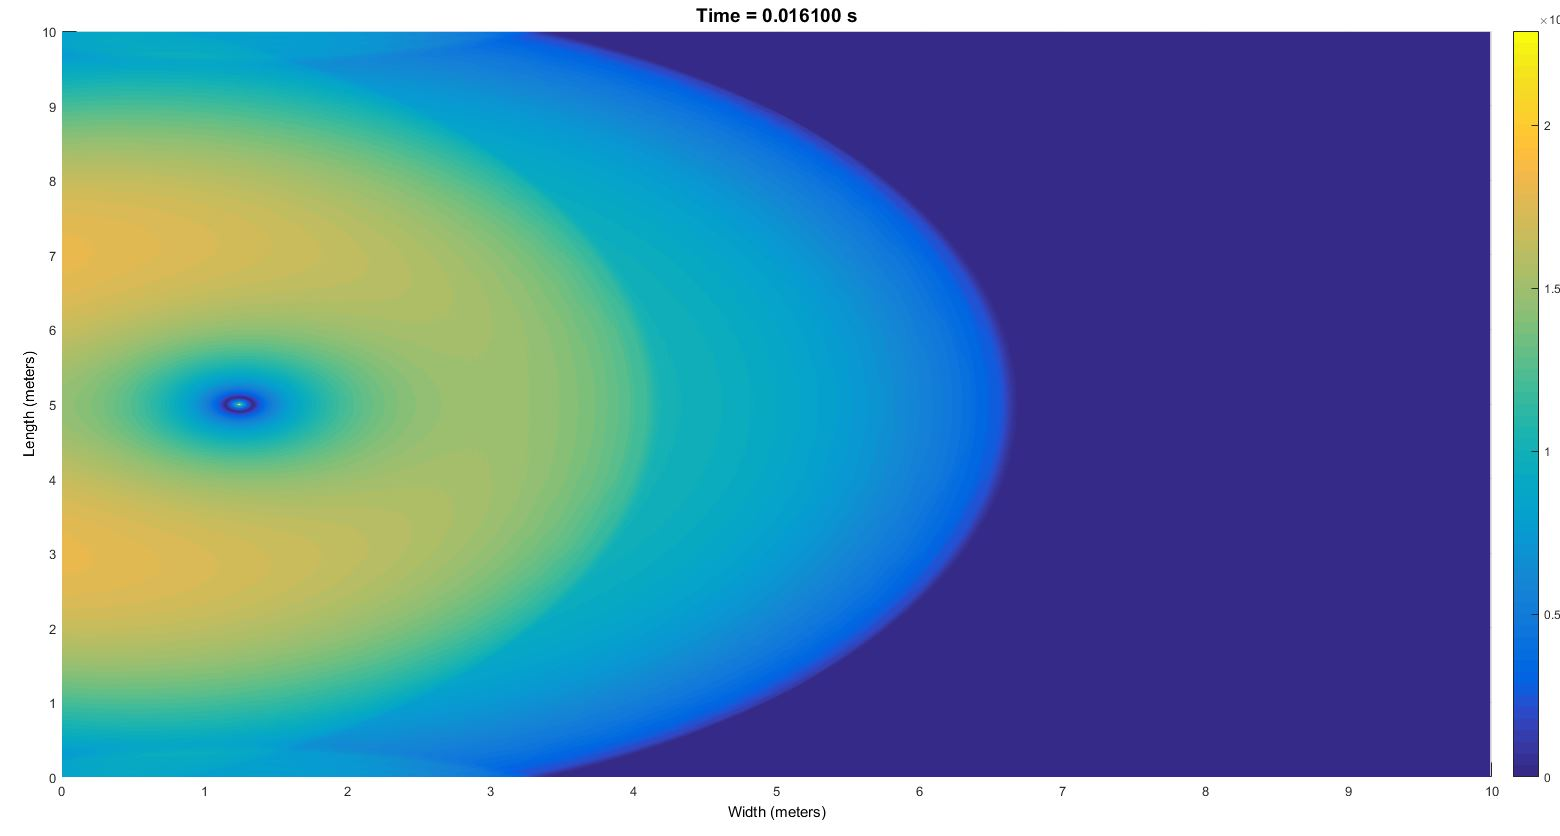
\includegraphics[width=0.6\textwidth]{explicit2dfdtd.jpg}
\centering
\caption{A visualisation of a 2D explicit FDTD simulation ~\cite{Durbridge2016a}}
\end{figure}

%\newpage

%------------------------------------------------
\section{Acoustic Modelling}
\subsection{Applications}
Acoustic modelling has a broad range of applications from the very large to the very small, and there are a number of key methods used to model different problem types. Problems of interest to this study are the acoustically large i.e. problems that are significantly large compared to a high proportion of the wavelengths of interest~\cite{Everest2009}. These problems could include multiple sources and receivers in spaces such as stadiums, cathedrals, shopping centres, caverns, cityscapes, mountain ranges etc.\\ For problems of this nature ray based modelling methods are commonly used, and have even been imlpemented for real-time simulation in video games~\cite{Bengtsson2009}. Ray based methods have a significant number of compromises, such as they do not accommodate for modal or atmospheric behaviour~\cite{Elorza2005}. Further to this when considering a large number of sound sources and receivers in a single large simulation, some of the benefits of ray based methods may be outweighed with computational cost. Wave based modelling methods have a similar set of benefits and drawbacks, that have as yet reduced use to high detail simulation of smaller problems. As higher computational power becomes more widely available, wave based methods may become more practical to use for problems with varying numbers of sources and receivers (particularly moving sources and receivers) e.g. video games, building acoustic demonstrations, personalised audio for viewing moving pictures, pilot training simulation etc. Below is a brief discussion of ray and wave based methods, with a deeper focus on time domain wave methods.
\begin{figure}
\centering
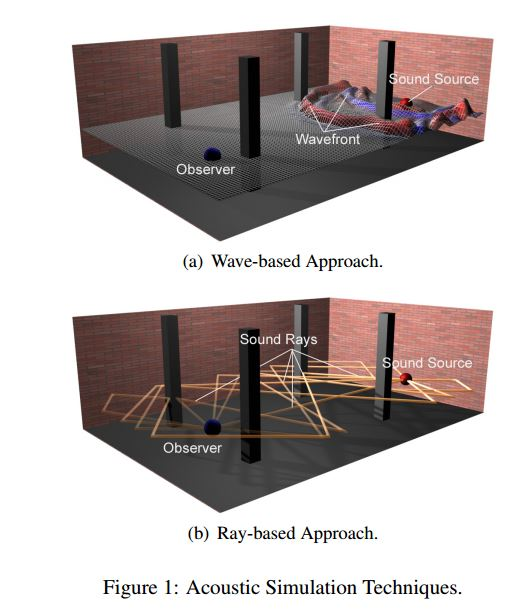
\includegraphics[width=0.5\textwidth]{simulationtechniques.jpg}
\centering
\caption{A visualisation of ray tracing~\cite{Rober2007}}
\end{figure} 

\subsection{Ray Methods}

Ray based modelling methods, also regarded as geometric methods, are those that rely on the concepts of ray physics in order to compute the impulse response of an acoustical system\footnote{In the context of this report, an acoustical system is the combination of sound source, sound receiver and surrounding environment}. In these methods (conceptually) rays are cast between sources and receivers, with the time of flight and boundary interactions(reflections) accounted for~\cite{Elorza2005}. As such this method relies on the assumption that the acoustic wavelength being modelled is significantly smaller than the smallest potential surface segment. Varieties of geometric methods include ray tracing, beam tracing and the image source model. These methods does not account for modal effects at low frequency~\cite{Rober2007}, and may require a significant number of rays for each source and receiver, in order for any result to be relevant for large problems. Further to this, a new model has to be computed every time a source and receiver moves to a different location or is 'aimed' in a different direction within the geometry. However, ray tracing is a relatively mature and well supported method in graphical rendering of environments, and may benefit from continual support and optimisation for faster performance~\cite{Rober2007}.


\subsection{Wave Methods}

Wave based modelling methods comprise of the discretization of a problem geometry into rational segments, following which a partial different equation is solved across the components or 'elements' of the geometry~\cite{Bilbao2004}. The partial different equations used in the context of large room acoustics problems are generally linearised Navier-Stokes equations for waves in homogeneous media~\cite{Rienstra1952a}. Some methods will compute solutions in the time domain i.e. iterative direct solutions, and some in the frequency domain such as FEM or the boundary element method(BEM). The benefit of 'element' methods such as FEM, BEM and Discontinuous Galerkin, is that a significant amount of supporting research has been done to improve this method of formulation for a wide range of physics problems~\cite{Zienkiewicz2013}. In acoustics, these methods still involve solving a domain that is discretized such that the smallest element is at least a sixth the size of the shortest wavelength of interest, and thus requires a significant amount of time to solve. Further more frequency domain calculations require solutions for every frequency of interest. Time domain methods for direct solutions can however be optimised for real time performance~\cite{Savioja2010}. Three variations of the finite difference time domain method are evaluated in the next section.

%------------------------------------------------
\section{The FDTD Method}
%---------------------------------------------

The explicit~\footnote{and by far most simple} finite-difference time domain(FDTD) method as conceived by Yee~\cite{Yee1966} for electromagnetics, involves discretizing a geometry into $N_d+1$ separate components where $N_d$. These components for an acoustic simulation are dimensional velocity fields $\textit{u}_{xyz}$, and an  inter-dimensionally uniform pressure grid $\textit{P}$. In the basic 7 point stencil for 2 dimensional simulation the time difference between the pressure and surrounding velocity gradients are a half step apart. The two differential components are evaluated in succession to determine velocities relative to pressure differentials, and then pressures values relative to surrounding velocities for completion of a single time step. This process is iterated over the whole time of the simulation~\cite{Schneider2015}.

\begin{figure}
\centering
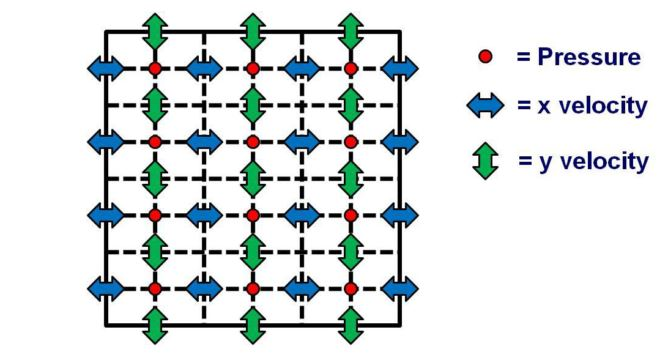
\includegraphics[width=0.6\textwidth]{2dexplicitfdtdexample.jpg}
\centering
\caption{A 2dimensional graph of the acoustic FDTD method in a basic rectangle geometry~\cite{Hill2012}}
\end{figure}

The generalised update equations for the generic 'leapfrog' acoustic finite difference time domain method in 3 dimensions are as follows~\footnote{these equations should be scaled out to calculate velocity in individual dimensions}

\begin{center}
$u_{xyz}(t + \frac{\delta t}{2}) = u_{xyz}(t - \frac{\delta t}{2}) - \frac{ \delta t}{\rho \delta d_{xyz}} [P_{2d_{xyz}}(t) - P_{d_{xyz}}(t)]$\\
$P_{xyz}(t + \delta t) = P_{xyz}(t) - \frac{ c^2 \rho \delta t}{ \delta d_{xyz}} [u_{2d_{xyz}}(t + \frac{\delta t}{2}) - u_{d_{xyz}}(t + \frac{\delta t}{2})]$\\
\end{center}
where:
\begin{enumerate}
\item $P =$ sound pressure
\item $u =$ velocity
\item $c =$ speed of sound
\item $\rho =$  material density
\item $d_{xyz}$ denotes spatial components 
\end{enumerate}

 The variation of FDTD described here is a second order central difference in space and first order forward difference in time~\footnote{calculating the future, based on the past and present}. For acceptable stability fulfilling the Courant condition~\cite{Abdulkadir2015}, upwards of 6 grid points per smallest wavelength is required per simulation~\cite{Oxnard2015}. FDTD 'stencils' often require a purely rectilinear discretization of the problem geometry~\footnote{thus not necessarily being accurate for round surfaces}, though octahedral and other schemes have been used in the similar finite-volume time domain method~\cite{Bilbao2016}. Although relatively simple and scalable, basic explicit FDTD methods require all calculations to be undertaken locally and as such are more prone to error as well as requiring a large number of memory accesses, however an implicit FDTD scheme may improve upon this performance~\cite{Hamilton2014}. As the stencil equations is identically replicated repeatedly within the problem geometry (excluding the boundaries), it is potentially highly parallelizable i.e. the same basic math operations are used to evaluate a large data set in fast succession~\cite{Savioja2010}~\cite{Angus2010}.

\subsection{S-FDTD}
The sparse finite difference time domain method is simply an extra step added~\cite{excluding some extra boundary handling to ensure stability} to the FDTD method, in which the power distribution of the grid is evaluated and only cells within a rational distance of those with an appropriate amount of energy are computed~\cite{Doerr2013}. This method is appropriate for electromagnetic simulation as the waves are transverse and can propagate through contiguous media (or no media) more simply than the acoustic case. As acoustic waves are longitudinal the SFDTD method may be applied to pulses such as Gaussian functions in order to still remain relevant, in this the travel and decay of wave fronts is accounted for in the calculation and multiple sources and receivers can be computed for simultaneously. Successful application of this method to acoustics is purely speculatory, as it has not been discussed so far in acoustics literature. 
\begin{figure}
\centering
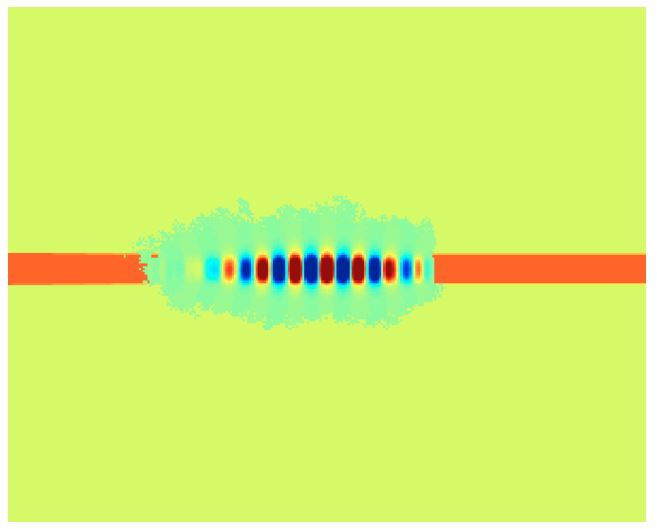
\includegraphics[width=0.6\textwidth]{sparsefdtd.jpg}
\centering
\caption{An example of SFDTD used to simulate a pic. The cloud represents the portion of the domain being computed ~\cite{Doerr2013}}
\end{figure}

\subsection{PSTD}
The pseudospectral time-domain method (PSTD) is a method of high accuracy frequency domain differentiation, with the simplicity and efficiency of time domain solving~\cite{Hornikx2016}. In this method, rows and columns are transformed into frequency domain representations, and are differentiated all together by being multiplied by a differentiating impulse response. The resulting grid is then evaluated with the appropriate coefficients and an attenuating perfectly-match layer is applied as an absorbing boundary condition~\cite{Angus2010}. There are three major benefits to the PSTD method over other methods:
\begin{enumerate}
\item Accuracy of the method is of the order $Nlog^N$
\item Differentiation undertaken across multiple points simultaneously speeds up computation
\item The speed an accuracy of FFT algorithms can be leveraged in this method for a greater reduction in computation time
\end{enumerate}

\begin{figure}
\centering
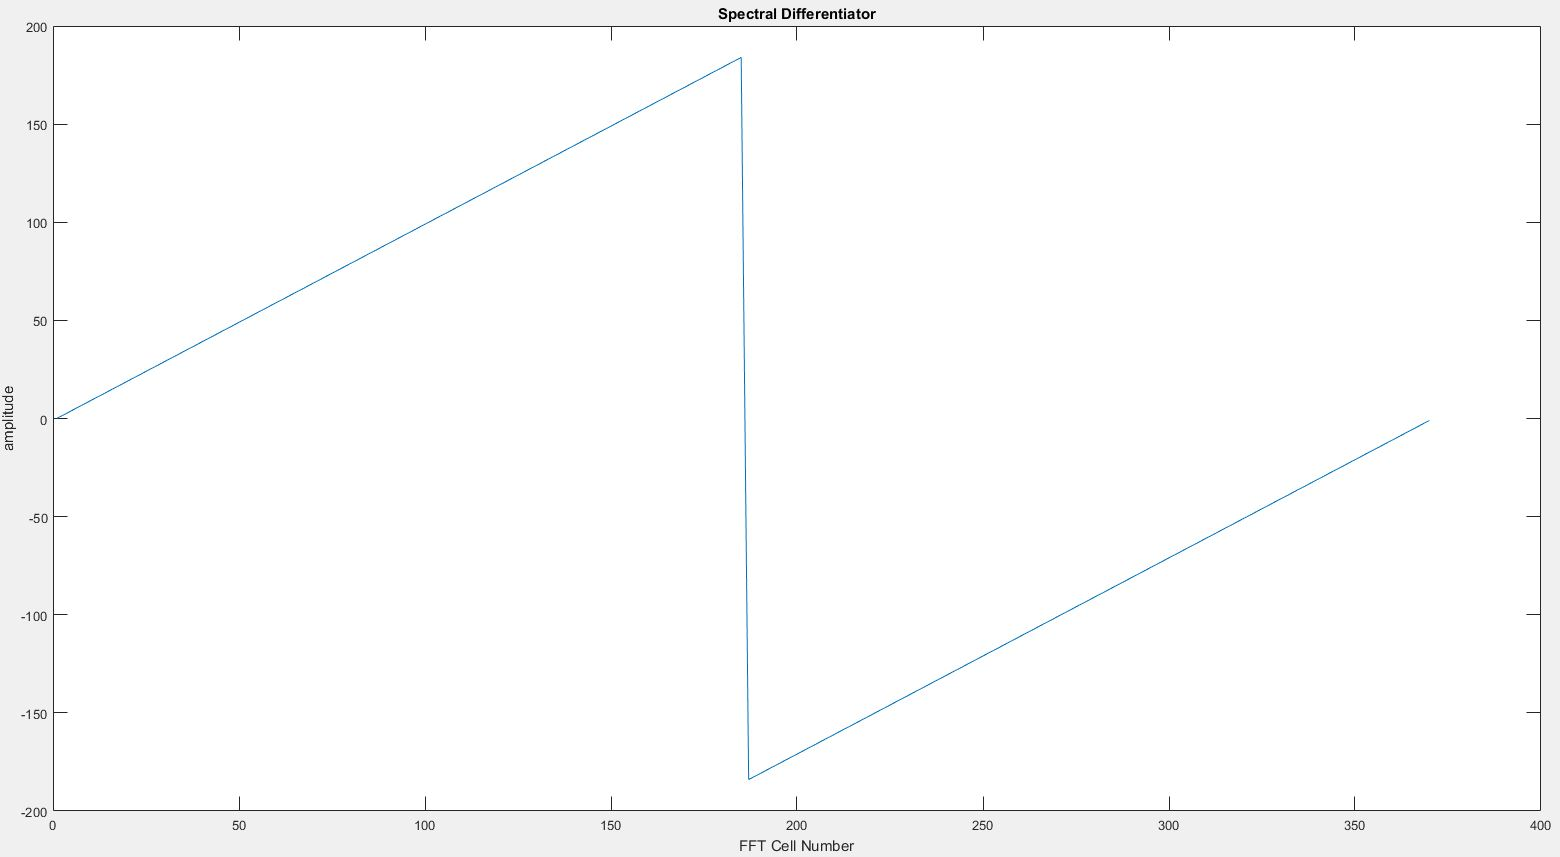
\includegraphics[width=0.5\textwidth]{spectraldiff.jpg}
\caption{Spectral Differentiator in the frequency domain~\cite{Durbridg2016}}
\end{figure}
\begin{figure}
\centering
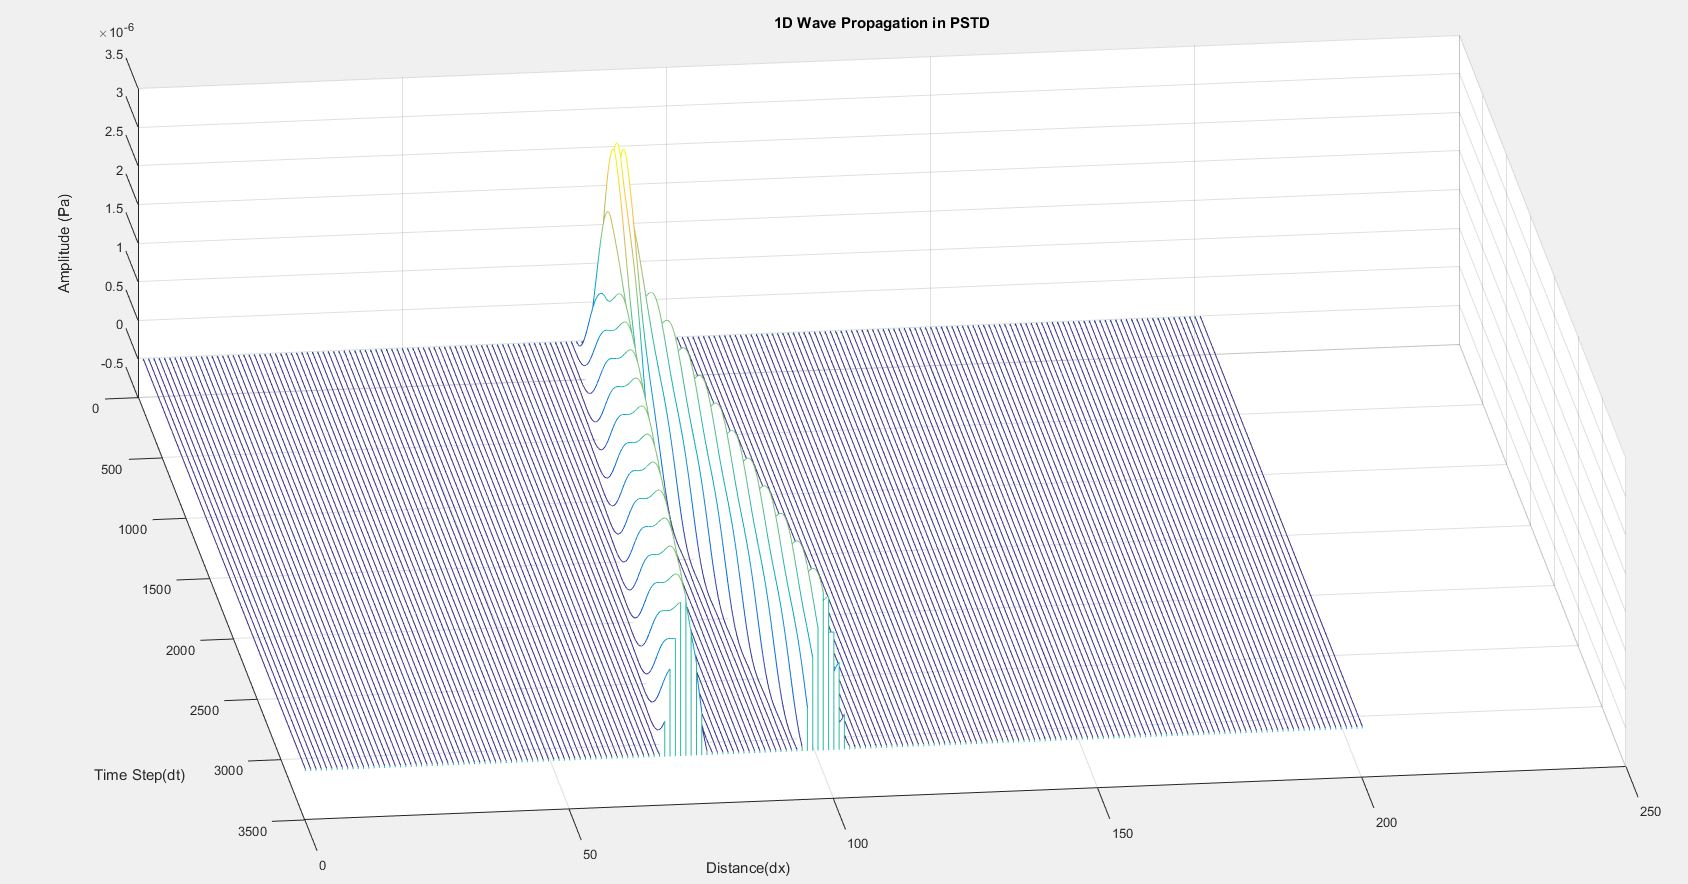
\includegraphics[width=0.5\textwidth]{pstdexamp.jpg}
\caption{Example 1D PSTD wave propagation~\cite{Durbridg2016}}
\end{figure}

\subsection{System Speed}
In order to obtain 'real time' performance in a non real time system such as a generic operating system, the modelling method must by able to receive, compute and return buffer-loads of audio samples in fast succession with minimal latency~\cite{Pirkle2013} i.e. having a system that performs optimally fast to allow for a minimal buffer size~\cite{Microsoft2016}. Direct solutions may be beneficial for very large problems with a large or fluctuating numbers of sources and receivers, as no extra computations will be necessary and the time distributed by the kernel can be used optimally for solution processing. An indirect solution may still be beneficial in some respects, as as system of indirect solutions can be cross-faded between~\cite{Galvez2016}. This means that if the computation process is 'running out of time', the previous solution can still be used. Although this solution is effectively 'incorrect' there will be less chance of returning a buffer without the correct number of results.

In Windows distributions before 10, the standard buffer size was 16mS which may equate to a 768 sample buffer. However, much of the buffer size is dependent on hardware drivers. As of Windows 10, buffer sizes default to 10mS i.e. 480 samples large~\cite{Microsoft2016}. However, as windows is a non-real time multi-tasking operating system, there is no trivial answer to how fast the process must perform beyond 'as fast as possible' with the largest problem size. Application on multiple GPGPUs may hold the key to ensuring operations occur fast enough for 'real-time' solutions~\cite{Savioja2010}. There is no 'hard and fast' way to determine how fast either algorithm must perform for all hardware and problem sizes on all computers.

%----------------------------------------------------------------------------------------
\section{Conclusion}
In this report, a description of acoustic modelling and some applications was given. The requirement for real time operation was suggested, and a basic description of modelling methods was given. The FDTD method was then described in more detail, along with two potential methods for increasing computation speed towards real time operation. In further work, the PSTD method and SFDTD methods would be applied and optimised in C++ and Cuda for the GPGPU. Some validation and benchmarking of problems would then take place, and a comparison made as to which method was more suited to real time operation with arbitrary sources and receivers.


%----------------------------------------------------------------------------------------
\section{References}

\bibliography{library}

\end{document}